%--------------------------------------------------------------------------
% 导入宏包
%--------------------------------------------------------------------------
\documentclass[•]{article}
\usepackage{CJKutf8}
\usepackage{graphicx}
\usepackage{xcolor}
\usepackage{color}
\usepackage{listings}%在Latex中插入代码块

%---------------------------------------------------------------------------
%文字超出边界的处理方法
\usepackage[textwidth=14.5cm]{geometry}
\usepackage{blindtext}  
\parindent=0pt  
%---------------------------------------------------------------------------

%--------------------------------------给文字加背景色--------------------------------
\usepackage{framed}
\colorlet{shadecolor}{gray!20}
%----------------------------------------------------------------------------------

%----------------------------------在Latex中插入代码块-------------------------------------
\lstset{
    basicstyle=\tt,
    %行号
    numbers=left,
    rulesepcolor=\color{red!20!green!20!blue!20},
    escapeinside=``,
    xleftmargin=2em,xrightmargin=2em, aboveskip=1em,
    %背景框
    framexleftmargin=1.5mm,
    frame=shadowbox,
    %背景色
    backgroundcolor=\color[RGB]{245,245,244},
    %样式
    keywordstyle=\color{blue}\bfseries,
    identifierstyle=\bf,
    numberstyle=\color[RGB]{0,192,192},
    commentstyle=\it\color[RGB]{96,96,96},
    stringstyle=\rmfamily\slshape\color[RGB]{128,0,0},
    %显示空格
    showstringspaces=false
}

%-------------------------------------总标题-------------------------------------
\title{Git}
%-------------------------------------latex上下间距-------------------------------------
\renewcommand{\baselinestretch}{1.5}
\begin{document}
\begin{CJK}{UTF8}{gbsn}
%-------------------------------------显示标题-------------------------------------
\maketitle

\section{Git简介}
\begin{center}
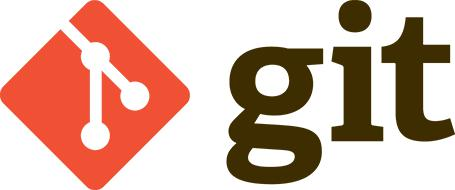
\includegraphics[scale=0.4]{0.jpeg}
\end{center}

\qquad \textbf{Git}是目前世界上最先进的分布式版本控制系统(没有之一)。Git有什么特点?简单来说就是:高端大气上档次!

\qquad \textcolor{red}{那什么是版本控制系统?}

\qquad 如果你用Microsoft Word写过长篇大论,那你一定有这样的经历:想删除一个段落,又怕将来想恢复找不回来怎么办?有办法,先把当前文件“另存为……”一个新的Word文件,再接着改,改到一定程度,再“另存为……”一个新文件,这样一直改下去,最后你的Word文档变成了这样:
\begin{center}
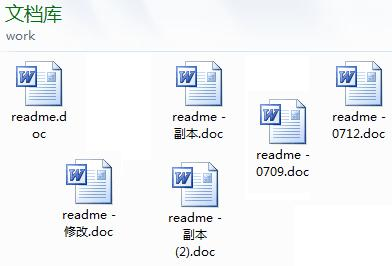
\includegraphics[scale=0.4]{1.jpeg}
\end{center}

\qquad 过了一周,你想找回被删除的文字,但是已经记不清删除前保存在哪个文件里了,只好一个一个文件去找,真麻烦。

\qquad 看着一堆乱七八糟的文件,想保留最新的一个,然后把其他的删掉,又怕哪天会用上,还不敢删,真郁闷。

\qquad 更要命的是,有些部分需要你的财务同事帮助填写,于是你把文件Copy到U盘里给她(也可能通过Email发送一份给她),然后,你继续修改Word文件。一天后,同事再把Word文件传给你,此时,你必须想想,发给她之后到你收到她的文件期间,你作了哪些改动,得把你的改动和她的部分合并,真困难。

\qquad 于是你想,如果有一个软件,不但能自动帮我记录每次文件的改动,还可以让同事协作编辑,这样就不用自己管理一堆类似的文件了,也不需要把文件传来传去。如果想查看某次改动,只需要在软件里瞄一眼就可以,岂不是很方便?

\qquad 这个软件用起来就应该像这个样子,能记录每次文件的改动:\\
\begin{center}
\begin{tabular}{ccccc}
\hline
版本& 文件名& 用户& 说明& 日期\\
\hline
1& service.doc& Male& 删除了软件服务条款5& 7/12 10:38\\
2& service.doc& Bill&  	增加了License人数限制& 7/12 10:38\\
3& service.doc& Steve& 删除了软件服务条款5& 7/12 10:38\\
4& service.doc& Jobs& 财务部门调整了合同金额& 7/12 10:38\\
5& service.doc& Gates& 延长了免费升级周期& 7/12 10:38\\
\hline\\
\end{tabular}
\end{center}

\qquad 这样,你就结束了手动管理多个“版本”的史前时代,进入到版本控制的20世纪。

\subsection{Git的诞生}

\qquad{很多人都知道,Linus在1991年创建了开源的Linux,从此,Linux系统不断发展,已经成为最大的服务器系统软件了。}

\qquad Linus虽然创建了Linux,但Linux的壮大是靠全世界热心的志愿者参与的,这么多人在世界各地为Linux编写代码,那Linux的代码是如何管理的呢?

\qquad 事实是,在2002年以前,世界各地的志愿者把源代码文件通过diff的方式发给Linus,然后由Linus本人通过手工方式合并代码!

\qquad 你也许会想,为什么Linus不把Linux代码放到版本控制系统里呢?不是有CVS、SVN这些免费的版本控制系统吗?因为Linus坚定地反对CVS和SVN,这些集中式的版本控制系统不但速度慢,而且必须联网才能使用。有一些商用的版本控制系统,虽然比CVS、SVN好用,但那是付费的,和Linux的开源精神不符。

\qquad 不过,到了2002年,Linux系统已经发展了十年了,代码库之大让Linus很难继续通过手工方式管理了,社区的弟兄们也对这种方式表达了强烈不满,于是Linus选择了一个商业的版本控制系统BitKeeper,BitKeeper的东家BitMover公司出于人道主义精神,授权Linux社区免费使用这个版本控制系统。

\qquad 安定团结的大好局面在2005年就被打破了,原因是Linux社区牛人聚集,不免沾染了一些梁山好汉的江湖习气。开发Samba的Andrew试图破解BitKeeper的协议(这么干的其实也不只他一个),被BitMover公司发现了(监控工作做得不错!),于是BitMover公司怒了,要收回Linux社区的免费使用权。

\qquad Linus可以向BitMover公司道个歉,保证以后严格管教弟兄们,嗯,这是不可能的。实际情况是这样的:

\qquad Linus花了两周时间自己用C写了一个分布式版本控制系统,这就是Git!一个月之内,Linux系统的源码已经由Git管理了!牛是怎么定义的呢?大家可以体会一下。

\qquad Git迅速成为最流行的分布式版本控制系统,尤其是2008年,GitHub网站上线了,它为开源项目免费提供Git存储,无数开源项目开始迁移至GitHub,包括jQuery,PHP,Ruby等等。

\qquad 历史就是这么偶然,如果不是当年BitMover公司威胁Linux社区,可能现在我们就没有免费而超级好用的Git了。

\subsection{集中式vs分布式}

\qquad Linus一直痛恨的CVS及SVN都是集中式的版本控制系统,而Git是分布式版本控制系统,集中式和分布式版本控制系统有什么区别呢?

\qquad 先说集中式版本控制系统,版本库是集中存放在中央服务器的,而干活的时候,用的都是自己的电脑,所以要先从中央服务器取得最新的版本,然后开始干活,干完活了,再把自己的活推送给中央服务器。中央服务器就好比是一个图书馆,你要改一本书,必须先从图书馆借出来,然后回到家自己改,改完了,再放回图书馆。
\begin{center}
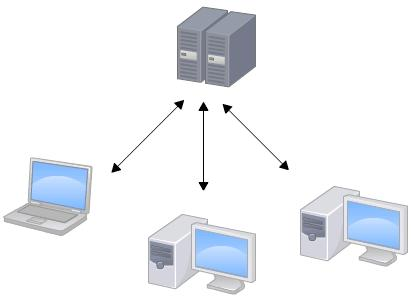
\includegraphics[scale=0.6]{2.jpeg}
\end{center}
\qquad 集中式版本控制系统最大的毛病就是必须联网才能工作,如果在局域网内还好,带宽够大,速度够快,可如果在互联网上,遇到网速慢的话,可能提交一个10M的文件就需要5分钟,这还不得把人给憋死啊。

\qquad 那分布式版本控制系统与集中式版本控制系统有何不同呢?首先,分布式版本控制系统根本没有“中央服务器”,每个人的电脑上都是一个完整的版本库,这样,你工作的时候,就不需要联网了,因为版本库就在你自己的电脑上。既然每个人电脑上都有一个完整的版本库,那多个人如何协作呢?比方说你在自己电脑上改了文件A,你的同事也在他的电脑上改了文件A,这时,你们俩之间只需把各自的修改推送给对方,就可以互相看到对方的修改了。

\qquad 和集中式版本控制系统相比,分布式版本控制系统的安全性要高很多,因为每个人电脑里都有完整的版本库,某一个人的电脑坏掉了不要紧,随便从其他人那里复制一个就可以了。而集中式版本控制系统的中央服务器要是出了问题,所有人都没法干活了。

\qquad 在实际使用分布式版本控制系统的时候,其实很少在两人之间的电脑上推送版本库的修改,因为可能你们俩不在一个局域网内,两台电脑互相访问不了,也可能今天你的同事病了,他的电脑压根没有开机。因此,分布式版本控制系统通常也有一台充当“中央服务器”的电脑,但这个服务器的作用仅仅是用来方便“交换”大家的修改,没有它大家也一样干活,只是交换修改不方便而已。
\begin{center}
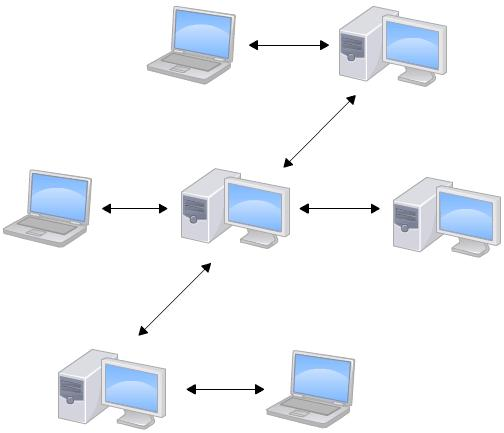
\includegraphics[scale=0.6]{3.jpeg}
\end{center}
\qquad 当然,Git的优势不单是不必联网这么简单,后面我们还会看到Git极其强大的分支管理,把SVN等远远抛在了后面。

\qquad CVS作为最早的开源而且免费的集中式版本控制系统,直到现在还有不少人在用。由于CVS自身设计的问题,会造成提交文件不完整,版本库莫名其妙损坏的情况。同样是开源而且免费的SVN修正了CVS的一些稳定性问题,是目前用得最多的集中式版本库控制系统。

\qquad 除了免费的外,还有收费的集中式版本控制系统,比如IBM的ClearCase(以前是Rational公司的,被IBM收购了),特点是安装比Windows还大,运行比蜗牛还慢,能用ClearCase的一般是世界500强,他们有个共同的特点是财大气粗,或者人傻钱多。

\qquad 微软自己也有一个集中式版本控制系统叫VSS,集成在Visual Studio中。由于其反人类的设计,连微软自己都不好意思用了。

\qquad 分布式版本控制系统除了Git以及促使Git诞生的BitKeeper外,还有类似Git的Mercurial和Bazaar等。这些分布式版本控制系统各有特点,但最快、最简单也最流行的依然是Git!
\section{安装Git}

\begin{sloppypar}  
\qquad 最早Git是在Linux上开发的,很长一段时间内,Git也只能在Linux和Unix系统上跑。不过,慢慢地有人把它移植到了Windows上。现在,Git可以在Linux、Unix、Mac和Windows这几大平台上正常运行了。
\end{sloppypar}
\qquad{\textbf{在Linux上安装Git}}

\qquad 首先,你可以试着输入git,看看系统有没有安装Git:

\lstset{language=C}
\begin{lstlisting}        %插入要显示的代码

$ git
The program 'git' is currently not installed. 
You can install it by typing:
sudo apt-get install git
\end{lstlisting}

\qquad 像上面的命令,有很多Linux会友好地告诉你Git没有安装,还会告诉你如何安装Git。如果你碰巧用Debian或Ubuntu Linux,通过一条{\color{red} sudo apt-get install git}就可以直接完成Git的安装,非常简单。

\qquad 老一点的Debian或Ubuntu Linux,要把命令改为{\color{red}sudo apt-get install git-core},因为以前有个软件也叫GIT(GNU Interactive Tools),结果Git就只能叫{\color{red}git-core}了。由于Git名气实在太大,后来就把GNU Interactive Tools改成{\color{red}gnuit,}{\color{red}git-core}正式改为{\color{red}git}。

\qquad 如果是其他Linux版本,可以直接通过源码安装。先从Git官网下载源码,然后解压,依次输入:{\color{red}./config},{\color{red}make}, {\color{red}sudo make install}这几个命令安装就好了。

安装完成后,还需要最后一步设置,在命令行输入:

\lstset{language=C}
\begin{lstlisting} 
$ git config --global user.name "Your Name"
$ git config --global user.email "email@example.com"
\end{lstlisting}

\qquad 因为Git是分布式版本控制系统,所以,每个机器都必须自报家门:你的名字和Email地址。你也许会担心,如果有人故意冒充别人怎么办?这个不必担心,首先我们相信大家都是善良无知的群众,其次,真的有冒充的也是有办法可查的。

\qquad 注意{\color{red} git config}命令的{\color{red}--global}参数,用了这个参数,表示你这台机器上所有的Git仓库都会使用这个配置,当然也可以对某个仓库指定不同的用户名和Email地址。

\begin{shaded}
参数,用了这个参数,表示你这台机器上所有的Git仓库都会使用这个配置,当然也可以对某个仓库指定不同的用户名和Email地址。
\end{shaded}



\section{创建版本库}
\qquad 什么是版本库呢?版本库又名仓库,英文名repository,你可以简单理解成一个目录,这个目录里面的所有文件都可以被Git管理起来,每个文件的修改、删除,Git都能跟踪,以便任何时刻都可以追踪历史,或者在将来某个时刻可以“还原”。

\qquad 所以,创建一个版本库非常简单,首先,选择一个合适的地方,创建一个空目录:
\lstset{language=C}
\begin{lstlisting} 
$ mkdir learngit
$ cd learngit
$ pwd
/Users/michael/learngit
\end{lstlisting}
\qquad \textbf{\color{red}pwd} 命令用于显示当前目录。在我的Mac上,这个仓库位于/Users/michael/learngit。

\qquad {\color{red}如果你使用Windows系统,为了避免遇到各种莫名其妙的问题,请确保目录名(包括父目录)不包含中文。}

\qquad 第二步,通过git init命令把这个目录变成Git可以管理的仓库:

\begin{lstlisting} 
$ git init
Initialized empty Git repository in /Users/learngit/.git/
\end{lstlisting}

\qquad 瞬间Git就把仓库建好了,而且告诉你是一个空的仓库(empty Git repository),细心的读者可以发现当前目录下多了一个.git的目录,这个目录是Git来跟踪管理版本库的,没事千万不要手动修改这个目录里面的文件,不然改乱了,就把Git仓库给破坏了。

\qquad 如果你没有看到.git目录,那是因为这个目录默认是隐藏的,用ls -ah命令就可以看见。

\qquad 也不一定必须在空目录下创建Git仓库,选择一个已经有东西的目录也是可以的。不过,不建议你使用自己正在开发的公司项目来学习Git,否则造成的一切后果概不负责。

\subsection{把文件添加到版本库} 

现在我们编写一个readme.txt文件,内容如下:

\begin{shaded}
Git is a version control system.\\
Git is free software.
\end{shaded}


\qquad 一定要放到learngit目录下(子目录也行),因为这是一个Git仓库,放到其他地方Git再厉害也找不到这个文件。

\qquad 和把大象放到冰箱需要3步相比,把一个文件放到Git仓库只需要两步。

\qquad 第一步,用命令git add告诉Git,把文件添加到仓库:
\begin{lstlisting} 
$ git add readme.txt/
\end{lstlisting}
\qquad 执行上面的命令,没有任何显示,这就对了,Unix的哲学是“没有消息就是好消息”,说明添加成功。

\qquad 第二步,用命令git commit告诉Git,把文件提交到仓库:
\begin{lstlisting} 
$ git commit -m "wrote a readme file"
[master (root-commit) eaadf4e] wrote a readme file
 1 file changed, 2 insertions(+)
 create mode 100644 readme.txt
\end{lstlisting}
\qquad 简单解释一下git commit命令,-m后面输入的是本次提交的说明,可以输入任意内容,当然最好是有意义的,这样你就能从历史记录里方便地找到改动记录。

\qquad 嫌麻烦不想输入-m "xxx"行不行?确实有办法可以这么干,但是强烈不建议你这么干,因为输入说明对自己对别人阅读都很重要。实在不想输入说明的童鞋请自行Google,我不告诉你这个参数。

\qquad git commit命令执行成功后会告诉你,1 file changed:1个文件被改动(我们新添加的readme.txt文件);2 insertions:插入了两行内容(readme.txt有两行内容)。
\qquad 为什么Git添加文件需要add,commit一共两步呢?因为commit可以一次提交很多文件,所以你可以多次add不同的文件,比如:
\begin{lstlisting} 
$ git add file1.txt
$ git add file2.txt file3.txt
$ git commit -m "add 3 files."
\end{lstlisting}

\subsection{小结}

现在总结一下今天学的两点内容:

初始化一个Git仓库,使用\fbox{\color{red}{git init}}命令。

添加文件到Git仓库,分两步:

    使用命令\fbox{\color{red}{git add <file>}},注意,可反复多次使用,添加多个文件;\\
    使用命令\fbox{\color{red}{git commit -m <message>}},完成。
    %-------------------\fbox{asd}%给文字加框
 


\section{版本管理}
\subsection{版本回退}
\subsection{工作区和缓存区}
\subsection{管理修改}
\subsection{删除文件}
\section{远程仓库}
\qquad 到目前为止,我们已经掌握了如何在Git仓库里对一个文件进行时光穿梭,你再也不用担心文件备份或者丢失的问题了。

\qquad 可是有用过集中式版本控制系统SVN的童鞋会站出来说,这些功能在SVN里早就有了,没看出Git有什么特别的地方。没错,如果只是在一个仓库里管理文件历史,Git和SVN真没啥区别。为了保证你现在所学的Git物超所值,将来绝对不会后悔,同时为了打击已经不幸学了SVN的童鞋,本章开始介绍Git的杀手级功能之一(注意是之一,也就是后面还有之二,之三……):远程仓库。

\qquad Git是分布式版本控制系统,同一个Git仓库,可以分布到不同的机器上。怎么分布呢?最早,肯定只有一台机器有一个原始版本库,此后,别的机器可以“克隆”这个原始版本库,而且每台机器的版本库其实都是一样的,并没有主次之分。

\qquad 你肯定会想,至少需要两台机器才能玩远程库不是?但是我只有一台电脑,怎么玩?其实一台电脑上也是可以克隆多个版本库的,只要不在同一个目录下。不过,现实生活中是不会有人这么傻的在一台电脑上搞几个远程库玩,因为一台电脑上搞几个远程库完全没有意义,而且硬盘挂了会导致所有库都挂掉,所以我也不告诉你在一台电脑上怎么克隆多个仓库。

\qquad 实际情况往往是这样,找一台电脑充当服务器的角色,每天24小时开机,其他每个人都从这个“服务器”仓库克隆一份到自己的电脑上,并且各自把各自的提交推送到服务器仓库里,也从服务器仓库中拉取别人的提交。

\qquad 完全可以自己搭建一台运行Git的服务器,不过现阶段,为了学Git先搭个服务器绝对是小题大作。好在这个世界上有个叫{\color{blue}{GitHub}}的神奇的网站,从名字就可以看出,这个网站就是提供Git仓库托管服务的,所以,只要注册一个GitHub账号,就可以免费获得Git远程仓库。
\qquad 在继续阅读后续内容前,请自行注册GitHub账号。由于你的本地Git仓库和GitHub仓库之间的传输是通过SSH加密的,所以,需要一点设置:

第1步:创建SSH Key。在用户主目录下,看看有没有.ssh目录,如果有,再看看这个目录下有没有\fbox{\color{red}{id-rsa}}和\fbox{\color{red}{id——rsa.pub}}这两个文件,如果已经有了,可直接跳到下一步。如果没有,打开Shell(Windows下打开Git Bash),创建SSH Key:

\begin{lstlisting} 
$ ssh-keygen -t rsa -C "youremail@example.com"
\end{lstlisting}

\qquad 你需要把邮件地址换成你自己的邮件地址,然后一路回车,使用默认值即可,由于这个Key也不是用于军事目的,所以也无需设置密码如果一切顺利的话,可以在用户主目录里找到\fbox{\color{red}{.ssh}}目录,里面有\fbox{\color{red}{id-rsa}}和\fbox{\color{red}{id-rsa.pub}}两个文件,这两个就是SSH Key的秘钥对,\fbox{\color{red}{id-rsa}}是私钥,不能泄露出去,\fbox{\color{red}{id-rsa.pub}}是公钥,可以放心地告诉任何人。

\qquad 第2步:登陆GitHub,打开“Account settings”,“SSH Keys”页面:

然后,点“Add SSH Key”,填上任意Title,在Key文本框里粘贴\fbox{\color{red}{id-rsa.pub}}文件的内容:

\begin{center}
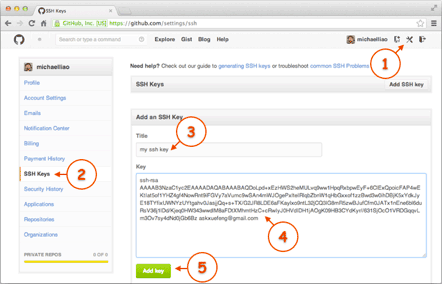
\includegraphics[scale=0.6]{add_ssh_key.png}
\end{center}

点“Add Key”,你就应该看到已经添加的Key:

\begin{center}
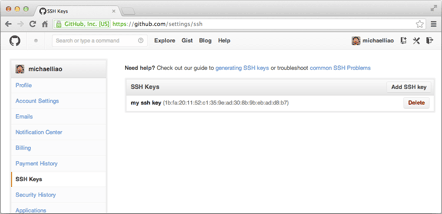
\includegraphics[scale=0.6]{add_key.png}
\end{center}

\qquad 为什么GitHub需要SSH Key呢?因为GitHub需要识别出你推送的提交确实是你推送的,而不是别人冒充的,而Git支持SSH协议,所以,GitHub只要知道了你的公钥,就可以确认只有你自己才能推送。当然,GitHub允许你添加多个Key。假定你有若干电脑,你一会儿在公司提交,一会儿在家里提交,只要把每台电脑的Key都添加到GitHub,就可以在每台电脑上往GitHub推送了。

\qquad 最后友情提示,在GitHub上免费托管的Git仓库,任何人都可以看到喔(但只有你自己才能改)。所以,不要把敏感信息放进去。

\qquad 如果你不想让别人看到Git库,有两个办法,一个是交点保护费,让GitHub把公开的仓库变成私有的,这样别人就看不见了(不可读更不可写)。另一个办法是自己动手,搭一个Git服务器,因为是你自己的Git服务器,所以别人也是看不见的。这个方法我们后面会讲到的,相当简单,公司内部开发必备。

确保你拥有一个GitHub账号后,我们就即将开始远程仓库的学习。

\subsection{添加远程仓库}
\qquad 现在的情景是,你已经在本地创建了一个Git仓库后,又想在GitHub创建一个Git仓库,并且让这两个仓库进行远程同步,这样,GitHub上的仓库既可以作为备份,又可以让其他人通过该仓库来协作,真是一举多得。
首先,登陆GitHub,然后,在右上角找到“Create a new repo”按钮,创建一个新的仓库:
\begin{center}
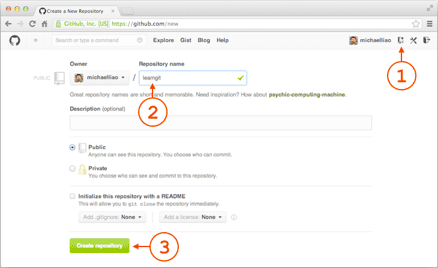
\includegraphics[scale=0.6]{4.png}
\end{center}
\qquad 在Repository name填入\fbox{\color{red}{learngit}} ,其他保持默认设置,点击“Create repository”按钮,就成功地创建了一个新的Git仓库:
\begin{center}
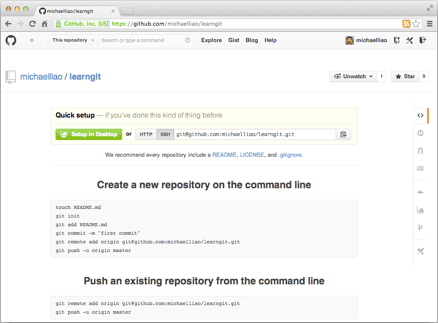
\includegraphics[scale=0.6]{5.png}
\end{center}
\qquad 目前,在GitHub上的这个\fbox{\color{red}{learngit}}仓库还是空的,GitHub告诉我们,可以从这个仓库克隆出新的仓库,也可以把一个已有的本地仓库与之关联,然后,把本地仓库的内容推送到GitHub仓库。

\qquad 现在,我们根据GitHub的提示,在本地的\fbox{\color{red}{learngit}}仓库下运行命令:
\begin{lstlisting} 
$ git remote add origin git@github.com:michaelliao/learngit.git
\end{lstlisting}

请千万注意,把上面的michaelliao替换成你自己的GitHub账户名,否则,你在本地关联的就是我的远程库,关联没有问题,但是你以后推送是推不上去的,因为你的SSH Key公钥不在我的账户列表中。

添加后,远程库的名字就是origin,这是Git默认的叫法,也可以改成别的,但是origin这个名字一看就知道是远程库。

下一步,就可以把本地库的所有内容推送到远程库上:

\subsection{从远程仓库克隆}
\section{分支管理}
\section{标签管理}
\section{使用GitHub}
\section{自定义Git}
\end{CJK}
\end{document}